\subsection{Räumliche Übersicht}
\label{sec:raeumliche_uebersicht}
%%%%%%%%%%%%%%%%%%%%%%%%%%%%%%%%%%%%%%%%%%%%%%%%%%%%%%%%%%%
%%%%%%%%%%%%%%%%%%%%%%%%%%%%%%%%%%%%%%%%%%%%%%%%%%%%%%%%%%%

Das \textbf{Telencephalon}\index{Telencephalon} (gelb) ist das rostralste Hirnareal (Abb.~\ref{fig:schaf_midsagittal}). In ihm verlaufen die lateralen Ventrikel (LV: Abb.~\ref{fig:schaf_midsagittal}~A, \ref{fig:schaf_lateral_sagittal}~B-L, \ref{fig:coronal_schaf}~C-H). Das Telencephalon beinhaltet die Großhirnrinde (Cx), die aus zwei Großhirnhemisphären besteht. Über die Fasern des Corpus callosum\index{Corpus! callosum} (cc) stehen die beiden Hemisphären miteinander in Verbindung (Abb.~\ref{fig:schaf_midsagittal}~A, \ref{fig:schaf_lateral_sagittal}~H, \ref{fig:coronal_schaf}~C-G). Anhand der Zellschichtung kann die Großhirnrinde in Neo-, Archi- und Paleocortex\index{Paleocortex} unterteilt werden. Am rostralen Ende des Gehirns befindet sich der Riechkolben (Bulbus olfactorius, OB)\index{Bulbus olfactorius}, der Teil des Riechhirns und somit des Paleocortex ist (Abb.~\ref{fig:schaf_midsagittal}~A, \ref{fig:schaf_lateral_sagittal}~I-J,
\ref{fig:coronal_schaf}~A-C). Der Neocortex\index{Neocortex} (NCx) ist eher superior-lateral gelegen. Er wird von der Fissura rhinalis (RF) räumlich vom eher inferior gelegenen Archicortex\index{Archicortex} (ACx) getrennt (Abb.~\ref{fig:coronal_schaf}~A-H). Ein Teilgebiet des Archicortex ist der cinguläre Cortex\index{Cortex! cinguli} (CCx). Dieser erstreckt sich von rostral nach caudal über dem Corpus callosum, dem Hippocampus und dem lateralen Ventrikel (Abb.~\ref{fig:schaf_lateral_sagittal}~K-L). Auch der Hippocampus\index{Hippocampus} (Hi) gehört zum Archicortex. Er ist medial im Telencephalon gelegen und umgibt c-förmig den Thalamus (Th) des Diencephalons (Abb.~\ref{fig:coronal_schaf}~G). Die Fimbria\index{Fimbria} (fi), eine schmale Faserstruktur, bildet am medialen Ende des Hippocampus den Beginn des Fornix\index{Fornix} (Abb.~\ref{fig:coronal_schaf}~G). Über die Fasern des Fornix (f) ist der Hippocampus mit dem inferior gelegenen Mammillarkörper (MB) verbunden (Abb.~\ref{fig:schaf_midsagittal}~B). Auch Teile der Basalganglia\index{Basalganglia} sind im Telencephalon lokalisiert. 
Dazu gehören beim Menschen und auch beim Schaf das Putamen und der Nucleus caudatus. 
Der Nucleus caudatus\index{Nucleus! caudatus} (Cu) ist medial im Telencephalon, unter dem cerebralen Cortex, gelegen. Er bildet einen Teil der lateralen Wand des lateralen Ventrikels (Abb.~\ref{fig:schaf_midsagittal}~C, \ref{fig:schaf_lateral_sagittal}~J-L, \ref{fig:coronal_schaf}~E-F). Das Putamen\index{Putamen} (CPu) liegt lateral, inferior und leicht rostral des Nucleus caudatus (\ref{fig:schaf_lateral_sagittal}~I, Abb.~\ref{fig:coronal_schaf}~D-F). Durch die Capsula externa (ec), die in die Capsula interna übergeht, sind beide Strukturen räumlich voneinander getrennt (Abb.~\ref{fig:coronal_schaf}~E). Bei Nagern und Nicht-Säugern ist aufgrund der weniger entwickelten Capsula interna keine Trennung von Putamen und Nucleus caudatus sichtbar. Man spricht dann vom sogenannten Caudoputamen-Komplex oder vom Striatum.\\
\noindent Das \textbf{Diencephalon}\index{Diencephalon} (orange) schließt sich caudal an das Telencephalon an und wird im superioren Bereich von diesem verdeckt. Es umschließt den dritten Ventrikel (3V), der mittig einen flachen Hohlraum im Gehirn bildet (Abb.~\ref{fig:schaf_midsagittal}~A,B, \ref{fig:coronal_schaf}~F-H). Von superior nach inferior kann das Diencephalon in Epithalamus, Thalamus, Subthalamus und Hypothalamus gegliedert werden. Die Epiphyse\index{Epiphyse} (Epi), als superiorster Teil des Zwischenhirns, gehört zum Epithalamus. Sie liegt caudal im Diencephalon, rostral der Vierhügelplatte, unter dem cerebralen Cortex (Abb.~\ref{fig:schaf_midsagittal}~D). Der Thalamus\index{Thalamus} (Th) bildet einen Teil der Wand des dritten Ventrikels. Er wird vom Hippocampus umschlungen (Abb.~\ref{fig:coronal_schaf}~G). Der Corpus geniculatum laterale\index{Corpus! geniculatum laterale} (LGN), eine Station der Sehbahn, ist superior im Thalamus gelegen. Ebenfalls Teil der Sehnbahn ist das Chiasma opticum\index{Chiasma opticum} (ox), an dem sich die optischen Trakte kreuzen. Diese Faserkreuzung befindet sich caudal des Thalamus und ist inferior an das Diencephalon angelagert (Abb.~\ref{fig:schaf_midsagittal}~A, \ref{fig:schaf_lateral_sagittal}J-L). Inferior des Thalamus, unter dem Subthalamus, liegt der Hypothalamus\index{Hypothalamus}. Er bildet die untere Wand des dritten Ventrikels. Ein Teilgebiet des Hypothalamus ist der Mammillarkörper\index{Mammillarkörper} (MB). Er liegt am inferioren Ende des Gehirns, caudal des optischen Chiasmas (Abb.~\ref{fig:schaf_midsagittal}~A,B).

\noindent Weiter caudal liegt das \textbf{Mesencephalon}\index{Mesencephalon} (blau). Es umschließt das Aqueductus mesencephali (Aq), das zwischen drittem und viertem Ventrikel liegt (Abb.~\ref{fig:schaf_midsagittal}~A,B). Innerhalb des Mesencephalons ist superior das Tectum gelegen. Es besteht aus der Vierhügelplatte\index{Vierhügelplatte}, die aus den superioren\index{Colliculus! superior} (SC) und inferioren Colliculi\index{Colliculus! inferior} (IC) aufgebaut ist. Die paarigen Colliculi superiores liegen rostral und superior der ebenfalls paarigen Colliculi inferiores (Abb.~\ref{fig:schaf_midsagittal}~D), \ref{fig:schaf_lateral_sagittal}~K-L, \ref{fig:coronal_schaf}~H-I). Unter dem Tectum liegt das Tegmentum mesencephali\index{Tegmentum! mesencephali} (Teg). Es befindet sich zwischen dem Mammillarkörper und dem Rhombencephalon (Abb.~\ref{fig:schaf_midsagittal}~A).

\noindent Das \textbf{Rhombencephalon}\index{Rhombencephalon} (grün) ist in Met- und Myelencephalon unterteilt. Im inferioren \textbf{Metencephalon}\index{Metencephalon} liegt der Pons\index{Pons} (Pn: Abb.~\ref{fig:schaf_midsagittal}~A, \ref{fig:coronal_schaf}~I-J). Im superioren Bereich des Metencephalons, über dem Pons, befindet sich das Cerebellum\index{Cerebellum! allgemein} (Cb: Abb.\ref{fig:schaf_midsagittal}~A). Es ist über die Fasern der Kleinhirnstiele oder Kleinhirn-Pedunkel\index{Kleinhirnpedunkel} (cp) mit Mesencephalon, Pons und Medulla verbunden (Abb.~\ref{fig:schaf_lateral_sagittal}~D-E, \ref{fig:coronal_schaf}~I). Die Kleinhirnsegel oder Veli\index{Velum} (ve) bilden das Dach des vierten Ventrikels (4V), der sich zwischen Pons und Cerebellum in rostro-caudaler Richtung erstreckt (Abb.~\ref{fig:schaf_midsagittal}~A, \ref{fig:coronal_schaf}~J). Das \textbf{Myelencephalon}\index{Myelencephalon} besteht aus der Medulla\index{Medulla oblongata} (Med), die caudal an den Pons angrenzt. Weiter caudal geht die Medulla in das Rückenmark\index{Rückenmark} (CS) über. Dabei geht der offene vierte Ventrikel, der superior entlang der Medulla verläuft, in den geschlossenen Zentralkanal des Rückenmarks über (Abb.~\ref{fig:schaf_midsagittal}~A,E, \ref{fig:coronal_schaf}~L).



\newpage
\subsubsection{Midsagittalschnitt}
\label{subsec:midsagittal}
%%%%%%%%%%%%%%%%%%%%%%%%%%%%%%%%%%%%%%%%%%%%%%%%%%%%%%%

\begin{figure}[H]
\centering
\begin{minipage}[b]{.8\textwidth}
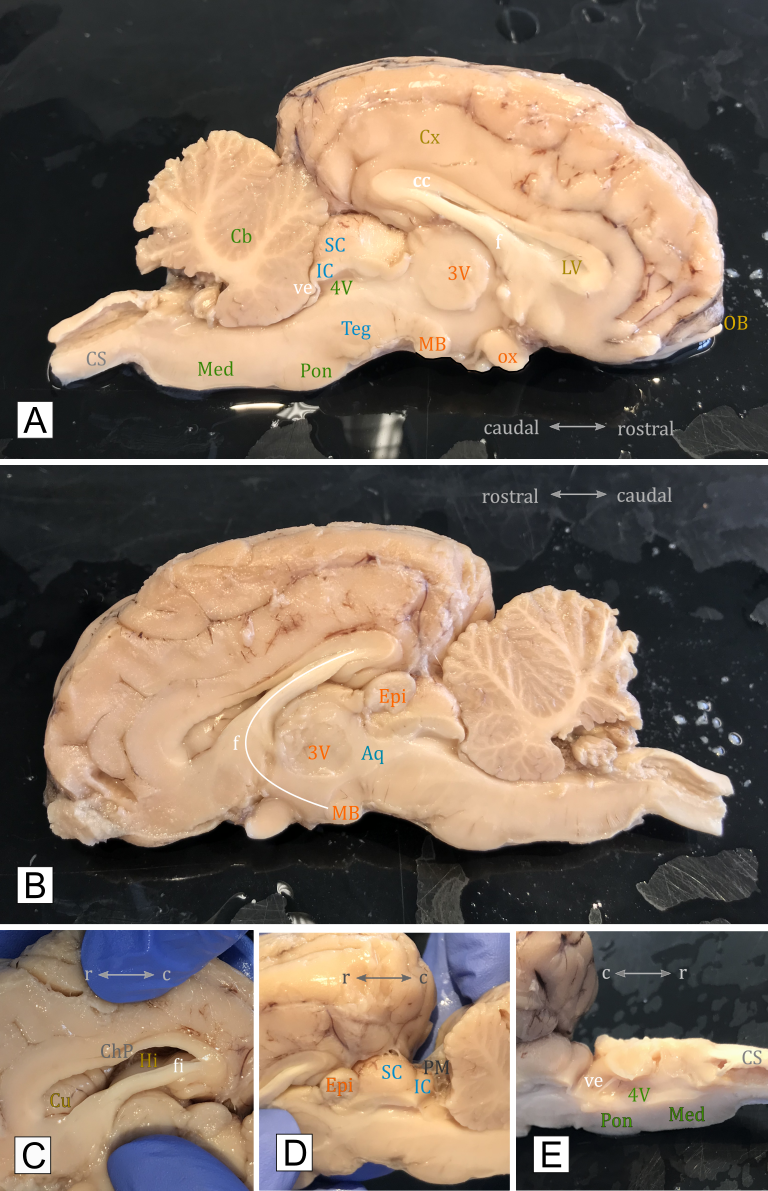
\includegraphics[width=\textwidth]{pictures/Bilder_Jule/Schaf/mittsagittal/schaf_mittsagittal_alle.png}
\end{minipage}
\caption[Midsagittalschnitt Schaf]{\textbf{Midsagittalschnitt Schaf. A}: linke Hemisphäre, \textbf{B}: rechte Hemisphäre, \textbf{C}: lateraler Ventrikel, \textbf{D}: Vierhügelplatte, \textbf{E}: Rhombencephalon ohne Cerebellum. Dabei ist in allen Bildern superior oben und inferior unten dargestellt. Bereiche, die dem Telencephalons zuzuordnen sind, sind gelblich bis bräunlich beschriftet, Bereiche des Diencephalons orange, des Mesencephalons blau und des Rhombencephalons grün. Fasern, bzw. Nerven sind mittels weißer Beschriftung gekennzeichnet.}
\label{fig:schaf_midsagittal}
\end{figure}


\newpage
\subsubsection{Laterale Sagittalschnitte}
\label{subsec:lateral_sagittal}
%%%%%%%%%%%%%%%%%%%%%%%%%%%%%%%%%%%%%%%%%%%%%%%%%%%%%%%

\begin{figure}[H]
    \centering
    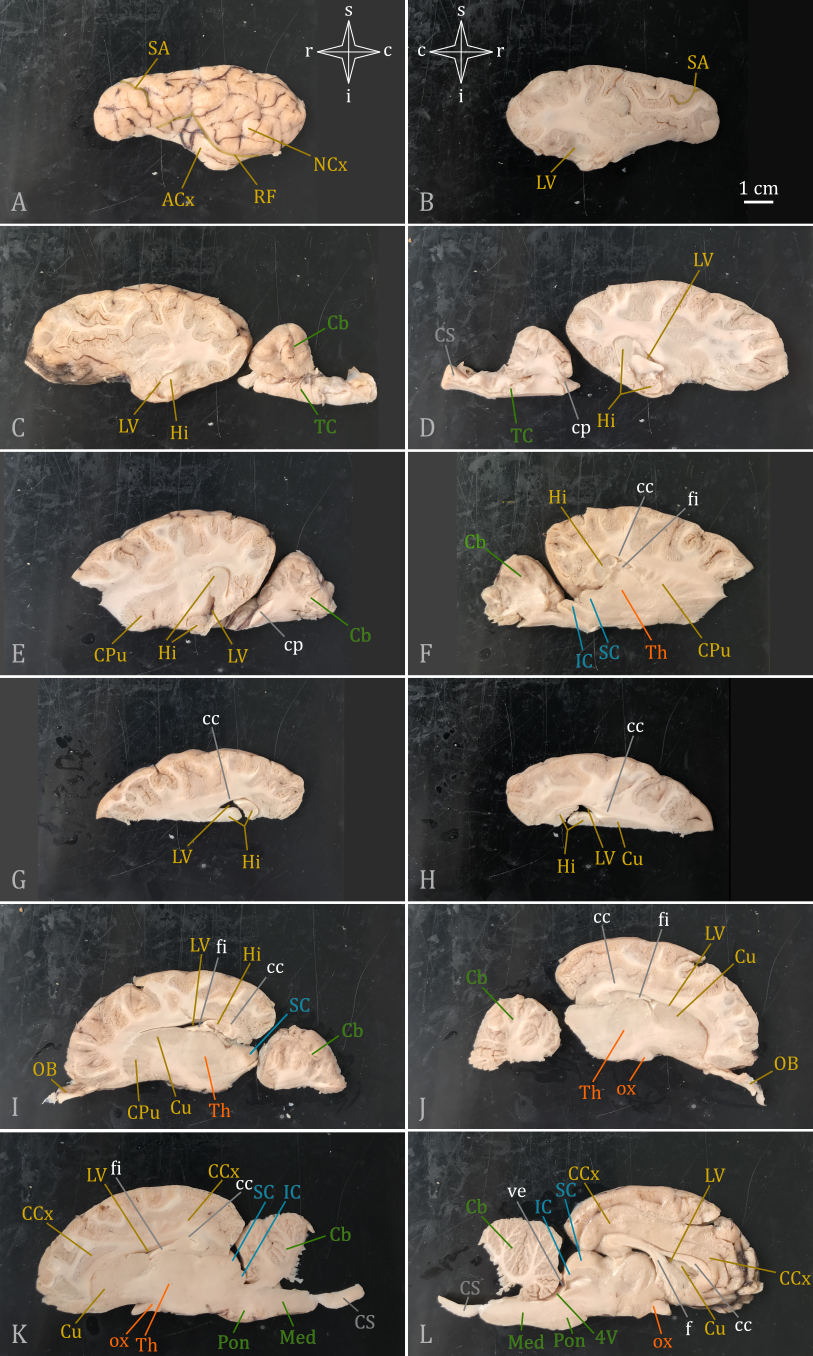
\includegraphics[width=0.8\textwidth]{pictures/Bilder_Jule/Schaf/lateral_sagittal/schaf_lateral_sagittal.png}
    \caption[Laterale Sagittalschnitte Schaf]{\textbf{Laterale Sagittalschnitte Schaf.} Die Schnitte sind von lateral (oben) nach medial (unten) angeordnet. Bereiche des Telencephalons sind gelb gekennzeichnet, Bereiche des Diencephalons orange, des Mesencephalons blau und des Rhombencephalons grün. Fasern sind weiß dargestellt.}
    \label{fig:schaf_lateral_sagittal}
\end{figure}


\newpage
\subsubsection{Coronalschnitte}
\label{subsec:coronal}
%%%%%%%%%%%%%%%%%%%%%%%%%%%%%%%%%%%%%%%%%%%%%%%%%%%%%%%

\begin{figure}[H]
\centering
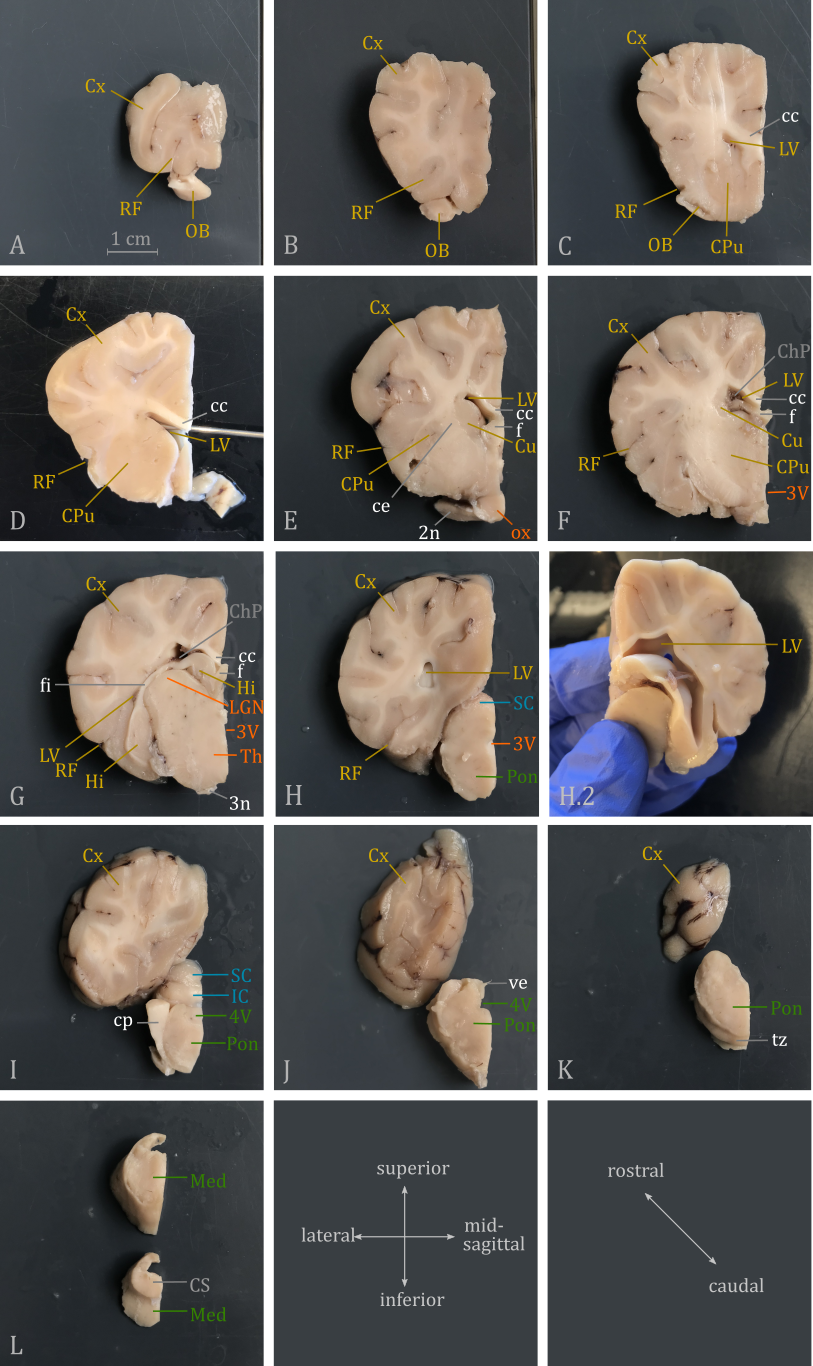
\includegraphics[width=0.8\textwidth]{pictures/Bilder_Jule/Schaf/coronal/coronal_schaf_all.png}
\caption[Coronalschnitte Schaf]{\textbf{Coronalschnitte Schaf.} Von rostral (links oben) nach caudal (rechts unten). Teilgebiete des Telencephalons sind gelb, des Diencephalons orange, des Mesencephalons blau und des Rhombencephalons grün beschriftet. Fasern, bzw. Nerven sind in weiß beschriftet.}
\label{fig:coronal_schaf}
\end{figure}

\subsubsection{Beschriftung und Kürzel}
%%%%%%%%%%%%%%%%%%%%%%%%%%%%%%%%%%%%%%%%%%%%%%%%%%%%%%%


\begin{table}[H]
\begin{tabular}{llcll}
           & 3V  & - & dritter Ventrikel                                                       & \multicolumn{1}{c}{\textbf{}} \\
\textbf{}  & 3n  & -          & Nervus oculomotorius                                                        & \multicolumn{1}{c}{}          \\
\textbf{}  & 4V  & -          & vierter Ventrikel                                                       & \multicolumn{1}{c}{}          \\
\textbf{A} & ACx & -          & Archicortex                                                             & \multicolumn{1}{c}{}          \\
\textbf{}  & Aq  & -          & Aquädukt, Aqueductus mesencephali, Aquaeductus cerebri                  & \multicolumn{1}{c}{}          \\
\textbf{C} & Cb  & - & Cerebellum, Kleinhirn                                                   & \multicolumn{1}{c}{\textbf{}} \\
           & cc  & - & Corpus callosum                                                         & \multicolumn{1}{c}{\textbf{}} \\
\textbf{}  & CCx & -          & cingulärer Cortex, Gyrus cinguli             & \multicolumn{1}{c}{}          \\
\textbf{}  & ce  & -          & Capsula externa                                                         & \multicolumn{1}{c}{}          \\
\textbf{}  & Chp & -          & Plexus choroideus                                                          & \multicolumn{1}{c}{}          \\
\textbf{}  & cp  & -          & Kleinhirn-Pedunkel                                                      & \multicolumn{1}{c}{}          \\
\textbf{}  & CPu & -          & Putamen                                                                 &                               \\
\textbf{}  & CS  & -          & Rückenmark                                                              &                               \\
\textbf{}  & Cu  & -          & Nucleus caudatus                                                        &                               \\
\textbf{}  & Cx  & -          & cerebraler Cortex, Cortex cerebri          &                               \\
\textbf{E} & Epi & -          & Epiphyse                                                                &                               \\
\textbf{F} & f   & -          & Fornix                                                                  &                               \\
\textbf{}  & fi  & -          & Fimbria                                                                 &                               \\
\textbf{H} & Hip & -          & Hippocampus                                                             &                               \\
\textbf{I} & IC  & -          & Colliculus inferior                                                     &                               \\
\textbf{L} & LGN & -          & Corpus geniculatum laterale                                             &                               \\
\textbf{}  & LV  & -          & lateraler Ventrikel                                                     &                               \\
\textbf{M} & MB  & -          & Mammillarkörper                                                         &                               \\
\textbf{}  & Med & -          & Medulla, Medulla oblongata                  &                               \\
\textbf{N} & NCx & -          & Neocortex                                                               &                               \\
\textbf{O} & OB  & -          & Riechkolben, Bulbus olfactorius                                                      &                               \\
\textbf{}  & ox  & -          & optisches Chiasma, Chiasma opticum           &                               \\
\textbf{P} & PM  & -          & Pia mater                                                               &                               \\
\textbf{}  & Pon & -          & Pons                                                                    &                               \\
\textbf{R} & RF  & -          & Fissura rhinalis                                                        &                               \\
\textbf{S} & SA  & -          & Sulcus ansatus                                                          &                               \\
\textbf{}  & SC  & -          & Colliculus superior                                                     &                               \\
\textbf{T} & TC  & -          & Hirnstamm, Truncus cerebri, Truncus encephali &                               \\
\textbf{}  & Teg & -          & Tegmentum, Tegmentum mesencephali           &                               \\
\textbf{}  & Th  & -          & Thalamus                                                                &                               \\
\textbf{}  & tz  & -          & Trapezkörper                                                            &                               \\
\textbf{V} & ve  & -          & Velum                                                                   &                              
\end{tabular}
\end{table}

